{
Denne udvidelse tager udgangspunkt i den eksisterende naive
fremgangsmåde, men søger at redefinere den idéelle position, for at en
region ligger i det gyldne snit. Hvor den naive fremgangsmåde tilgodeser
regioner som ligger op ad snittet, leder vi nu efter regioner som i
højere grad er centreret på snittet. Vi leder nu efter regioner med
massemidtpunkt i det gyldne snit, og kigger ikke længere på denne
regions begrænsende rektangel. Et eksempel på dette kan ses i
figur \ref{hus}, hvor den sorte region ikke anses som liggende i det
gyldne snit af den naive fremgangsmåde, men vi vil gerne have, at sådanne
regioner, klassificeres som en positive, interessante regioner.

\begin{figure}[h]
	\begin{center}
		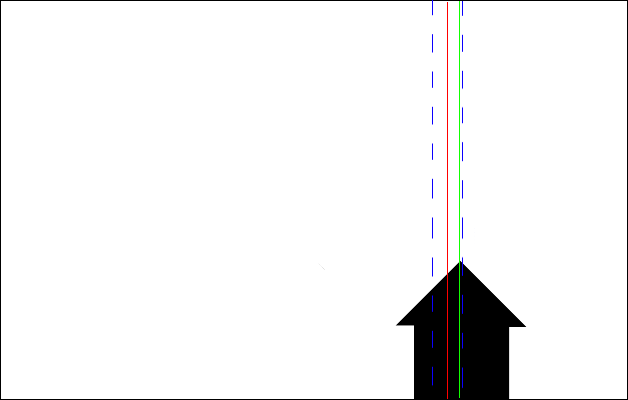
\includegraphics[scale=0.3,angle=0]{afsnit/vores_implementation/billeder/udvidet_loesning/husworks.png}
	\end{center}
	\caption[]{Et hus som bliver skåret over, så midten ligger inde for
    snittets margin.}
	\label{hus}
\end{figure}

\subsubsection{Opdeling af region med et gitter}
Vi bruger ikke længere regionens begrænsende rektangel, til at beskrive
regionen, så har vi brug for en anden måde at repræsentere denne på. Vi
laver derfor en approksimation, af regionens form og udstrækning, ved at
bruge et gitter.  Alt efter hvor finmasket dette gitter er, kan man
justere hvor præcis approksimationen af regionen skal være. Et eksempel
på et gitter, ses i figur \ref{grid}, hvor regionen beskrives ved de
punkter, hvor to linjer krydser, og befinder sig inden for regionen.

I praksis bruges det segmenterede billede fra floodfill-metoden, til at
konstruere regionens approksimation. Vi kontrollerer hver pixel, som er
en del af gitteret, i det begrænsende rektangel for en given region, om
denne har samme farve, som regionen er blevet tildelt. Vi finder da et
undersæt af punkter til at beskrive regionen.

\begin{figure}[h]
    \centering
    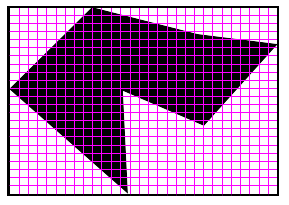
\includegraphics[scale=0.76,angle=0]{afsnit/vores_implementation/billeder/udvidet_loesning/udvidetloesninglayer.png}
    \caption[]{Et gitter over en regions begrænsende rektangel.}
    \label{grid}
\end{figure}

\subsubsection{Bedømmelse med hensyn til massemidtpunkt}
Givet en region $R$ betegner vi antallet af punkter i regionen med
$|R|$. Vi antager, at vi betragter et vertikalt snit $G$ i et billede.
Det gælder, for alle punkter $p \in R$, at de kan befinde sig ovenpå,
til højre eller til venstre for $G$. I denne sammenhæng lader vi $R_r$
og $R_l$ beskrive punkter, henholdsvis til højre og venstre for snittet
$G$.  Afstanden fra et punkt til kanten af et billede kaldes $D_p$, hvor
kanten er origo i billedet.

Med disse informationer, kan vi afgøre, om snittet deler regionen i to
lige store dele, samt om store dele af regionen, befinder sig langt væk
fra snittet. Vi vil gerne kigge på en regions massemidtpunkt, og se om
dette ligger inden for margin.

\begin{definition}
    En regions massemidtpunkt er givet ved
    \begin{eqnarray}
        m(R) & = & \frac{\sum_{p \in R}{D_p}}{|R|} \label{masssemidpunkt}
        \label{MPunkt}
    \end{eqnarray}
    hvor $m(R)$ giver os en værdi for, hvilken lige linje, der deler
    regionen op i to dele, som er mest ens.
    \label{def_massemidtpunkt}
\end{definition}

\begin{figure}[h]
    \begin{center}
        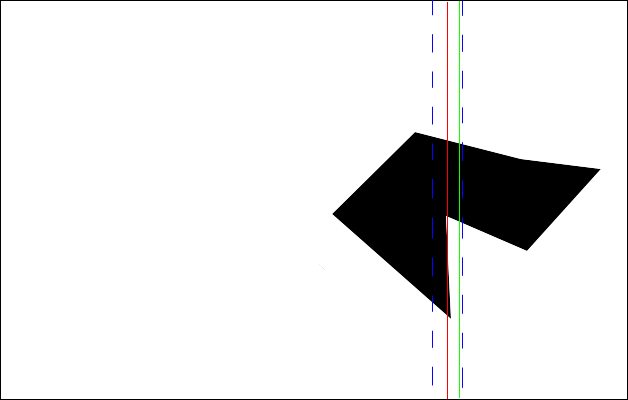
\includegraphics[scale=0.5,angle=0]{afsnit/vores_implementation/billeder/udvidet_loesning/cOMCutMargin.png}
    \end{center}
    \caption[]{Region, hvor massemidtpunkt, snit og margin er tegnet
    ind. Det ses, at massemidtpunktet, tegnet med en grøn linje, ligger
    inde for margin.}
    \label{cOMCutMargin}
\end{figure}

Hvis $m(R)$ ligger inden for margin, som tilfældet i figur
\ref{cOMCutMargin}, siger vil vi gerna have at regionen klassificeres
som positiv. Det er imidlertid ikke nok, kun at bedømme regionerne efter
massemidtpunkt, da man kan konstruere regioner, som vi ikke vil godtage,
men som har massemidtpunkt inden for margin. Et eksempel på en sådan
region er vist i figur \ref{dontwork}, hvor selve fordelingen af
regionens masse er skæv.

\begin{figure}[h]
    \begin{center}
        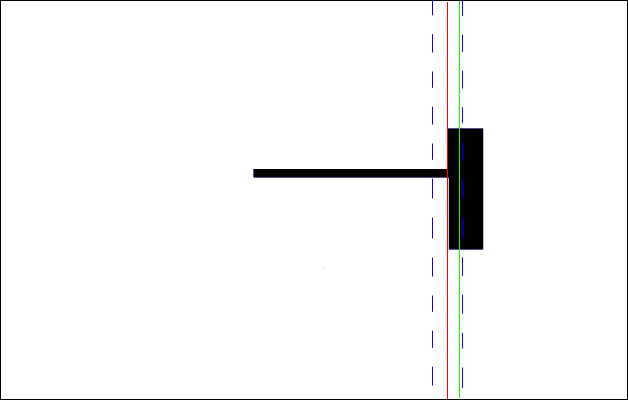
\includegraphics[scale=0.5,angle=0]{afsnit/vores_implementation/billeder/udvidet_loesning/dontWork.png}
    \end{center}
    \caption[]{Region, som har massemidtpunkt inden for margin, men som
    ikke kvalificerer sig til at ligge i snittet pga. arealets
    fordeling.}
    \label{dontwork}
\end{figure}

Vi forsøger at løse dette problem, ved at kontrollere regionens
fordeling over snittet.

\begin{definition}
    En regions fordeling over snittet findes ved
    \begin{eqnarray}
        f(R) & = & \frac{|R_{l}| - |R_{r}|}{|R|}
        \label{Fordeling}
    \end{eqnarray}
    \label{def_fordeling_ligning}
\end{definition}

\begin{definition}
    En region er jævnt fordelt over snittet, hvis forholdet mellem
    punkterne, på den højre og venstre side, er lavere en $0.75$.
    \label{def_fordeling_procent}
\end{definition}

I \eqref{Fordeling} sammenlignes antal punkter, på begge sider af
snittet, og giver en procentsats for, hvor stor forskel der er mellem
siderne. Vi har at $f(R) \in [-1,1]$.  Hvis $f(R)$ er positiv, er der
$f(R)$ procent flere punkter på venstre side og vice versa. Her vises
netop hvorfor denne fremgangsmåde adskiller sig markant fra den naive.
Den naive fremgangsmåde søger nemlig at udvælge de regioner $R$, hvor
størstedelen af punkter ligger på den ene side af snittet, dvs. $|f(R)|
\geq 0.75$. Den udvidede løsning gør nøjagtig det modsatte og finder
regioner som er jævnt fordelt over snittet.

Vi bruger nu ovenstående til at definere, hvornår en region ligger i
snittet.

\begin{definition}
    Hvis en region er jævnt fordelt over snittet og har et
    massemidtpunkt inden for margin, så ligger denne region i snittet.
    \label{def_expanded}
\end{definition}

% Fjernet, da dette vil være første gang vi viser et egentligt resultat.
% Man ved ikke hvad man ser. Sådanne billeder bør vente til afprøvning.
%
%Få
%at give et eksempel på hvornår vores naive algoritme virker, se figur \ref{centerOfMass}
%\begin{figure}[h]
%	\begin{center}
%		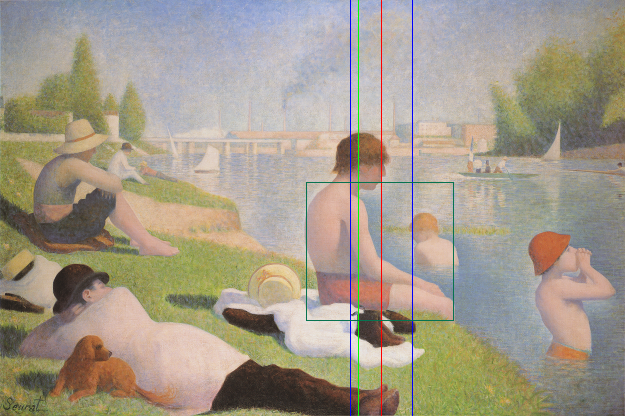
\includegraphics[scale=0.35,angle=0]{afsnit/vores_implementation/billeder/udvidet_loesning/centerOfMass.png}
%	\end{center}
%	\caption[]{Eksempel på hvordan den udvidet algoritme virker på et billedet hvor den naive algoritme ikke vil have fundet det}
%	\label{centerOfMass}
%\end{figure}

}

% vim: set tw=72 spell spelllang=da:
